% ======================================================================
%  REPORTE FINAL - ENTREGABLE 3
%  Reto MA2008B - Optimizacion No Lineal - OXXO Planogramacion
%
%  Figuras tomadas de ../outputs/ (ver \graphicspath):
%    resultados_ga1.png, resultados_ga2.png, planograma_bco.png,
%    convergencia_BCO_CF_4.0_Refrescos.png, criterios_BCO_CF_4.0_Refrescos.png
%  Compilar con pdflatex (2 pasadas para indice y referencias).
% ======================================================================
\documentclass[11pt,letterpaper]{article}

\usepackage[utf8]{inputenc}
\usepackage[T1]{fontenc}
\usepackage{lmodern}
\usepackage[spanish,es-tabla]{babel}
\usepackage{microtype}

\usepackage{amsmath, amssymb, amsthm}
\usepackage{mathtools}
\usepackage{geometry}
\usepackage{graphicx}
\usepackage{booktabs}
\usepackage{array}
\usepackage{multirow}
\usepackage{colortbl}
\usepackage{caption}
\usepackage{subcaption}
\usepackage{float}
\usepackage{enumitem}
\usepackage{algorithm}
\usepackage{algpseudocode}
\usepackage{xcolor}
\usepackage{titlesec}
\usepackage{fancyhdr}
\usepackage{hyperref}

% ---- geometria y colores de marca --------------------------------------
\geometry{margin=2.4cm}
\definecolor{oxxored}{RGB}{197,11,33}
\definecolor{oxxodark}{RGB}{38,38,46}
\definecolor{headgray}{gray}{0.92}
\graphicspath{{../outputs/}{./}}

\hypersetup{colorlinks=true, linkcolor=oxxored, urlcolor=oxxored,
            citecolor=oxxored, pdftitle={Reto OXXO - Entregable 3},
            pdfauthor={Equipo MA2008B}}

% ---- estilo de titulos de seccion --------------------------------------
\titleformat{\section}{\Large\bfseries\color{oxxored}}{\thesection}{0.6em}{}[{\color{oxxored!40}\titlerule[1pt]}]
\titleformat{\subsection}{\large\bfseries\color{oxxodark}}{\thesubsection}{0.5em}{}
\titlespacing*{\section}{0pt}{1.4em}{0.6em}

% ---- encabezado y pie --------------------------------------------------
\pagestyle{fancy}
\fancyhf{}
\fancyhead[L]{\small\color{oxxodark}Reto OXXO\,\textendash\,Entregable 3}
\fancyhead[R]{\small\color{oxxodark}Optimizaci\'on de Planogramas}
\fancyfoot[C]{\small\thepage}
\renewcommand{\headrulewidth}{0.4pt}
\renewcommand{\footrulewidth}{0pt}

% ---- estilo de captions y tablas ---------------------------------------
\captionsetup{font=small, labelfont={bf,color=oxxored}, labelsep=period}
\renewcommand{\arraystretch}{1.22}
\newcommand{\thead}[1]{\rowcolor{headgray}#1}

\title{\vspace{-1.5em}}
\begin{document}

% ======================================================================
%  PORTADA
% ======================================================================
\begin{titlepage}
\centering
\vspace*{1.2cm}
{\color{oxxored}\rule{\linewidth}{2pt}}\\[0.5cm]
{\Huge\bfseries\color{oxxodark} Optimizaci\'on de Planogramas\\[0.25em]
en Tiendas OXXO\par}
\vspace{0.5cm}
{\Large Entregable 3: Experimentaci\'on y Resultados\par}
\vspace{0.2cm}
{\large Reto MA2008B\,\textendash\,Optimizaci\'on No Lineal\par}
{\color{oxxored}\rule{\linewidth}{2pt}}\\[1.4cm]

{\large\bfseries Equipo\par}
\vspace{0.4cm}
\begin{tabular}{ll}
Daniel Eugenio Gonz\'alez Limas    & A01285898 \\
Sebasti\'an Zaragoza D\'iaz        & A01286211 \\
Cedrick Patricio Trevi\~no Ortiz   & A01198868 \\
Lillianne Sep\'ulveda Cuevas       & A00839109 \\
Juan Fernando Gonz\'alez Cervantes & A01571586 \\
Javier Rojas Orrante               & A01352213 \\
\end{tabular}

\vfill
{\large IDM, 6to Semestre\par}
{\large Instituto Tecnol\'ogico y de Estudios Superiores de Monterrey\par}
\vspace{0.6cm}
\href{https://github.com/DanielLaBanda/RETO_OXXO_OPTINL}{\texttt{github.com/DanielLaBanda/RETO\_OXXO\_OPTINL}}
\vspace{1cm}
\end{titlepage}

% ======================================================================
%  RESUMEN E INDICE
% ======================================================================
\begin{abstract}
\noindent Este trabajo aborda el problema de \emph{planogramaci\'on} de tiendas
OXXO: dada la asignaci\'on de productos y sus frentes (decidida en etapas previas
del proceso comercial), se determina la ubicaci\'on \'optima de cada producto
dentro de un mueble de cuarto fr\'io. Se presenta un algoritmo gen\'etico (en dos
variantes, no extendida y extendida) y se compara contra un modelo no lineal tipo
\emph{random-key} resuelto por \textbf{evoluci\'on diferencial} (\emph{Differential
Evolution}), sobre cuatro formatos de planograma reconstruidos del hist\'orico. La
funci\'on objetivo, no lineal por su t\'ermino de varianza, maximiza aprovechamiento
de espacio, coherencia de tama\~no y agrupaci\'on de marca. El algoritmo gen\'etico
supera tanto al acomodo experto hist\'orico como al modelo no lineal en los cuatro
formatos, con aprovechamiento de espacio entre 90.9\,\% y 95.7\,\%.
\end{abstract}

{\small\tableofcontents}
\thispagestyle{fancy}
\newpage

% ======================================================================
\section{Introducci\'on y contexto}
% ======================================================================
El proceso de surtido de OXXO consta de cuatro etapas: segmentaci\'on de la tienda,
asignaci\'on de espacio por categor\'ia, definici\'on de variedad y
\textbf{planogramaci\'on}. Este trabajo se ubica en la \'ultima: el tama\~no del
mueble y la lista de productos con sus frentes \emph{ya est\'an decididos}, y solo
resta ubicar cada producto en su charola y posici\'on. Por ello el modelo no
maximiza ventas (decididas aguas arriba) sino la \textbf{calidad del acomodo},
medida como una combinaci\'on de aprovechamiento de espacio, coherencia de tama\~no
y agrupaci\'on de marca.

El objetivo del entregable es \textbf{experimentar} con el modelo: resolver el
problema con un algoritmo gen\'etico (GA), contrastarlo con un modelo de
optimizaci\'on no lineal sobre las mismas instancias, y validar los resultados
contra el acomodo hist\'orico real de OXXO.

% ======================================================================
\section{Modelo matem\'atico}
% ======================================================================
\subsection{Conjuntos, par\'ametros y variables}
\textbf{Conjuntos:} $P=\{1,\dots,N\}$ bloques-producto a colocar; $S=\{1,\dots,M\}$
charolas del mueble (con $M=6\cdot\text{TAMA\~NO}$); $B$ marcas.\\[0.2em]
\textbf{Par\'ametros:} $a_j=\text{ANCHO}_j\times\text{frentes}_j$ (ancho del bloque,
cm), $h_j$ (alto, cm), $W=55$ cm (ancho \'util de charola en cuarto fr\'io),
$\text{SEP}=0.5$ cm (separador entre productos), $w_1,w_2,w_3$ (pesos),
$\rho$ (penalizaci\'on por charola excedente) y
$P(\text{charola}\mid j)$ (distribuci\'on hist\'orica de ubicaci\'on).\\[0.2em]
\textbf{Variables:} $x_{ij}\in\{0,1\}$ (bloque $j$ en charola $i$) y
$p_{ij}\in\mathbb{Z}_{\ge0}$ (posici\'on dentro de la charola). El modelo no lineal
usa adem\'as $y_j\in[0,1]$, una llave continua (\emph{random-key}) que induce el
orden de colocaci\'on.

\subsection{Funci\'on objetivo (no lineal)}
\begin{equation}
\max\; Z \;=\; w_1\,U \;-\; w_2\,C_{\text{tam}} \;+\; w_3\,B_{\text{marca}}
\;-\; \rho\cdot\max\!\bigl(0,\; M_{\text{usadas}}-M\bigr)
\label{eq:obj}
\end{equation}
donde $U$ es el aprovechamiento promedio de ancho de las charolas usadas,
$C_{\text{tam}}$ la incoherencia de tama\~no (desviaci\'on est\'andar del alto dentro
de cada charola; t\'ermino \textbf{no lineal} por involucrar varianzas) y
$B_{\text{marca}}$ la fracci\'on de productos contiguos que comparten marca. La
restricci\'on dura es la capacidad de ancho con separadores:
\begin{equation}
\sum_{j\in P} a_j\, x_{ij} \;+\; \text{SEP}\,(n_i-1) \;\le\; W
\qquad \forall\, i\in S,
\label{eq:cap}
\end{equation}
con $n_i$ el n\'umero de bloques en la charola $i$. El modelo extendido (GA2) a\~nade
un t\'ermino $+\,w_4\,L$ que premia colocar cada producto cerca de su charola
esperada hist\'orica.

\subsection{M\'etodo heur\'istico: algoritmo gen\'etico}
Cada individuo es una \textbf{permutaci\'on} de los $N$ bloques. Se decodifica con un
esquema \emph{first-fit}: se recorren los bloques en el orden de la permutaci\'on y
se colocan en la charola actual mientras quepan (Ec.~\eqref{eq:cap}); al no caber, se
abre la siguiente. As\'i toda permutaci\'on es factible en ancho por construcci\'on y
solo se penaliza el exceso de charolas.

\begin{algorithm}[H]
\caption{Algoritmo gen\'etico para el acomodo de planograma}
\begin{algorithmic}[1]
\State Inicializar poblaci\'on (50\,\% sembrada por altura con ruido, 50\,\% aleatoria)
\For{cada generaci\'on}
  \State Evaluar el fitness de cada individuo (Ec.~\eqref{eq:obj})
  \State Conservar la \'elite
  \While{poblaci\'on incompleta}
    \State padres $\gets$ selecci\'on por torneo ($k=3$)
    \State hijo $\gets$ OX(padres);\quad hijo $\gets$ mutar(hijo)
    \State agregar hijo
  \EndWhile
\EndFor
\State \textbf{return} mejor individuo encontrado
\end{algorithmic}
\end{algorithm}

\subsection{Modelo no lineal de comparaci\'on (\emph{random-key})}
Para contrastar el algoritmo gen\'etico se implement\'o un modelo de optimizaci\'on
no lineal con codificaci\'on \emph{random-key}: cada bloque $j$ tiene una variable
continua $y_j\in[0,1]$; al ordenar los valores $y_j$ se obtiene una permutaci\'on que
el \emph{mismo} decodificador first-fit del GA convierte en charolas. La funci\'on
objetivo es la misma de la Ec.~\eqref{eq:obj}, por lo que la comparaci\'on es directa
y aisla el \emph{m\'etodo de b\'usqueda}. Como la funci\'on $Z(y)$ no es suave ni
convexa (por la desviaci\'on est\'andar de alturas y las adyacencias de marca), se
resolvi\'o con \textbf{evoluci\'on diferencial} (\emph{Differential Evolution},
\texttt{scipy.optimize}), un optimizador global sin derivadas que opera sobre el
vector continuo de llaves.

% ======================================================================
\section{Procesamiento de datos y valores esperados}
% ======================================================================
El socio formador proporcion\'o un dataset hist\'orico de $\approx$497k filas de
planogramas de \emph{Refrescos} en cuarto fr\'io, que agrega m\'ultiples tiendas. El
preprocesamiento (\texttt{preprocessing/pipeline\_.py}) consta de cuatro pasos.

\begin{description}[leftmargin=1.4em, style=nextline, itemsep=0.35em]
\item[1. Clave de planograma.] Se agrupa por SEGMENTO $+$ MUEBLE $+$ TAMA\~NO $+$
PLANOGRUPO. Las direcciones DI/ID son el mismo dise\~no espejado, por lo que se
reconstruye desde la direcci\'on dominante.
\item[2. Reconstrucci\'on por bloques-producto.] El dataset no contiene ID de tienda:
cada posici\'on est\'a observada $\sim$95 veces (tiendas apiladas). Cada
\texttt{UBICACION\_BANDEJA} es un \emph{frente}, no un producto. Por cada
(charola, frente) se toma el UPC modal del hist\'orico y se colapsan frentes
consecutivos del mismo producto en bloques (frentes $=$ n\'umero de bandejas,
ancho $=$ ANCHO $\times$ frentes). As\'i se obtiene un planograma can\'onico realista
en lugar del universo agregado del formato.
\item[3. Distribuci\'on y valor esperado de ubicaci\'on.] Cada producto no tiene una
charola fija, sino una \textbf{distribuci\'on de probabilidad}
$P(\text{charola}\mid\text{producto})$, estimada contando en cu\'antas tiendas
apareci\'o en cada nivel. Su media es el \textbf{valor esperado de ubicaci\'on}
$E[\text{charola}]$ (Secci\'on~\ref{sec:eubic}); es el insumo del t\'ermino $w_4$ de
GA2.
\item[4. Pesos por simulaci\'on.] En lugar de fijar $w_1,w_2,w_3$ a mano, se estiman
por simulaci\'on: en cada uno de 1000 escenarios se muestrea un UPC por frente seg\'un
$P(\text{UPC}\mid\text{posici\'on})$, se arma un planograma plausible y se miden los
tres criterios. El valor esperado y la desviaci\'on de cada criterio determinan los
pesos mediante $w_k\propto E[\text{criterio}_k]/\sigma[\text{criterio}_k]$
(relaci\'on se\~nal/ruido), normalizados a escala 3.
\end{description}

\paragraph{Artefactos y validaci\'on.} El pipeline produce por formato tres archivos
en \texttt{data/}: \texttt{oxxo\_instance\_*.csv} (bloques con dimensiones, frentes,
marca y $E[\text{charola}]$), \texttt{oxxo\_locdist\_*.json} (distribuci\'on de
charola por producto) y \texttt{oxxo\_weights\_*.json} (pesos simulados con sus
desviaciones y un campo de validaci\'on). El GA y el modelo no lineal consumen
exactamente la misma instancia. Se valid\'o autom\'aticamente que cada planograma
tuviera un n\'umero de productos realista, charolas iguales al nominal del formato,
ancho por charola $\le 55$ cm (con tolerancia) y un solo producto por posici\'on:
\textbf{132 de 132 planogramas} pasaron la validaci\'on.

% ======================================================================
\section{Tama\~no del problema}
% ======================================================================
El problema se representa como un \textbf{grafo bipartito de asignaci\'on}
producto--charola: hay un nodo por cada bloque-producto y un nodo por cada charola,
de modo que $|V|=|P|+|S|$; cada posible asignaci\'on de un producto a una charola es
un arco, $|A|=|P|\cdot|S|$. La formulaci\'on \emph{random-key} optimiza $|P|$
variables continuas (una llave por producto); su equivalente discreto tendr\'ia una
variable binaria $x_{ij}$ por arco ($|P|\cdot|S|$). Los par\'ametros son
$a_j,h_j,b_j$ por bloque m\'as los globales $W,\text{SEP},w_1,w_2,w_3,\rho$, esto es
$3|P|+6$.

\begin{table}[H]
\centering\small
\begin{tabular}{lrrrrr}
\toprule
\thead{\textbf{Formato}} & \textbf{Nodos} & \textbf{Arcos} &
\textbf{Var.\ NLP} & \textbf{Var.\ grafo} & \textbf{Par\'am.} \\
& {\small$|P|+|S|$} & {\small$|P|\cdot|S|$} & {\small$|P|$} &
{\small$|P|\cdot|S|$} & {\small$3|P|+6$} \\
\midrule
SIN\_CFC\_1.0 \,(27p/6c)   & 33  & 162  & 27  & 162  & 87  \\
OFC\_CF\_2.0 \,(67p/12c)   & 79  & 804  & 67  & 804  & 207 \\
BCO\_CF\_4.0 \,(101p/24c)  & 125 & 2424 & 101 & 2424 & 309 \\
OFC\_CF\_5.5 \,(156p/32c)  & 188 & 4992 & 156 & 4992 & 474 \\
\bottomrule
\end{tabular}
\caption{Dimensiones del problema por formato.}
\label{tab:size}
\end{table}

% ======================================================================
\section{Experimentaci\'on y resultados}
% ======================================================================
\subsection{Entorno de c\'omputo}
\begin{table}[H]
\centering\small
\begin{tabular}{ll}
\toprule
\thead{\textbf{Componente}} & \textbf{Especificaci\'on} \\
\midrule
Modelo de la PC        & MacBook Air (Apple Silicon) \\
Sistema operativo      & macOS Tahoe 26.5 \\
Memoria RAM            & 16 GB \\
Software               & Python 3.13.13 (un solo hilo) \\
Librer\'ias            & numpy 2.4.6, pandas 3.0.3, scipy 1.17.1, \\
                       & Pillow 12.2.0, matplotlib 3.10.9 \\
Modelo no lineal       & Random-key $+$ Differential Evolution (\texttt{scipy.optimize}) \\
\bottomrule
\end{tabular}
\caption{Entorno de c\'omputo utilizado.}
\end{table}

\subsection{Supuestos}
\begin{itemize}[leftmargin=1.6em, itemsep=0.2em]
\item Los frentes son un dato dado por el socio; no se optimizan.
\item Ancho \'util de charola $=55$ cm (cuarto fr\'io); separador de $0.5$ cm solo
entre productos, no en los bordes.
\item El planograma se reconstruye con el UPC modal por posici\'on; es una
aproximaci\'on estad\'istica (ver limitaciones).
\item Las direcciones DI/ID se tratan como espejo de un mismo dise\~no.
\end{itemize}

\subsection{Configuraci\'on de los algoritmos}
\begin{table}[H]
\centering\small
\begin{tabular}{ll@{\hskip 2.2em}ll}
\toprule
\multicolumn{2}{l}{\textbf{Algoritmo gen\'etico}} &
\multicolumn{2}{l}{\textbf{Modelo no lineal (random-key)}} \\
\midrule
Poblaci\'on  & 150           & Representaci\'on & $y_j\in[0,1]$ continua \\
Generaciones & 400           & Decodificador    & First-fit (igual al GA) \\
Elitismo     & 8             & B\'usqueda       & Evoluci\'on diferencial (DE) \\
Selecci\'on  & Torneo, $k=3$ & Estrategia       & \texttt{best1bin}, recomb.\ 0.7 \\
Cruce        & OX            & Poblaci\'on DE   & $8\cdot N$ \\
Mutaci\'on   & 0.2           & Evaluaciones     & hasta $\sim$309k \\
Semilla      & 42            & Semilla          & 7 \\
\bottomrule
\end{tabular}
\caption{Configuraci\'on del GA y del modelo no lineal. Ambos optimizan la misma
funci\'on objetivo y usan el mismo decodificador, por lo que sus fitness son
directamente comparables.}
\end{table}

\subsection{Comparaci\'on por formato: Hist\'orico vs.\ GA vs.\ NLP}
La Tabla~\ref{tab:comp} resume el desempe\~no de los tres enfoques en los cuatro
formatos, sobre la misma instancia y la misma funci\'on objetivo.

\begin{table}[H]
\centering\small
\begin{tabular}{llrrrrrrr}
\toprule
\thead{\textbf{Formato}} & \textbf{M\'etodo} & \textbf{Fit.} & \textbf{Aprov.\%} &
\textbf{Desp.\%} & \textbf{Incoh.} & \textbf{Marca\%} & \textbf{Char.} &
\textbf{$t$(s)} \\
\midrule
\multirow{3}{*}{\shortstack[l]{BCO\_CF\_4.0\\{\footnotesize 101p/24c}}}
  & Hist\'orico    & 2.349 & 88.5 & 11.5 & 1.72 & 55.8 & 24 & --- \\
  & \cellcolor{headgray}\textbf{GA} & \cellcolor{headgray}\textbf{2.442} & \cellcolor{headgray}92.4 & \cellcolor{headgray}7.6 & \cellcolor{headgray}2.24 & \cellcolor{headgray}59.0 & \cellcolor{headgray}23 & \cellcolor{headgray}11.9 \\
  & NLP rnd-key    & 2.323 & 92.4 & 7.6 & 5.01 & 25.6 & 23 & 31.2 \\
\midrule
\multirow{3}{*}{\shortstack[l]{SIN\_CFC\_1.0\\{\footnotesize 27p/6c}}}
  & Hist\'orico    & 2.092 & 75.6 & 24.4 & 1.00 & 57.1 & 6 & --- \\
  & \cellcolor{headgray}\textbf{GA} & \cellcolor{headgray}\textbf{2.526} & \cellcolor{headgray}90.9 & \cellcolor{headgray}9.1 & \cellcolor{headgray}3.42 & \cellcolor{headgray}81.8 & \cellcolor{headgray}5 & \cellcolor{headgray}3.9 \\
  & NLP rnd-key    & 2.476 & 90.9 & 9.1 & 5.96 & 77.3 & 5 & 2.1 \\
\midrule
\multirow{3}{*}{\shortstack[l]{OFC\_CF\_2.0\\{\footnotesize 67p/12c}}}
  & Hist\'orico    & 2.418 & 90.6 & 9.4 & 1.82 & 56.4 & 12 & --- \\
  & \cellcolor{headgray}\textbf{GA} & \cellcolor{headgray}\textbf{2.462} & \cellcolor{headgray}90.6 & \cellcolor{headgray}9.4 & \cellcolor{headgray}1.25 & \cellcolor{headgray}72.7 & \cellcolor{headgray}12 & \cellcolor{headgray}7.7 \\
  & NLP rnd-key    & 2.328 & 90.6 & 9.4 & 4.57 & 40.0 & 12 & 18.4 \\
\midrule
\multirow{3}{*}{\shortstack[l]{OFC\_CF\_5.5\\{\footnotesize 156p/32c}}}
  & Hist\'orico    & 2.119 & 80.6 & 19.4 & 1.54 & 51.6 & 32 & --- \\
  & \cellcolor{headgray}\textbf{GA} & \cellcolor{headgray}\textbf{2.502} & \cellcolor{headgray}95.7 & \cellcolor{headgray}4.3 & \cellcolor{headgray}1.61 & \cellcolor{headgray}51.2 & \cellcolor{headgray}27 & \cellcolor{headgray}15.8 \\
  & NLP rnd-key    & 2.329 & 95.7 & 4.3 & 5.80 & 17.1 & 27 & 80.9 \\
\bottomrule
\end{tabular}
\caption{Comparaci\'on de los tres enfoques por formato (Refrescos, cuarto fr\'io).
El GA obtiene el mayor fitness en los cuatro casos. Incoh.\ $=$ desviaci\'on
est\'andar media de altura por charola (cm); Marca $=$ \% de adyacencias de la misma
marca; Char.\ $=$ charolas usadas (sin sobrecupo en ning\'un caso).}
\label{tab:comp}
\end{table}

\paragraph{Lectura.} El algoritmo gen\'etico \textbf{supera tanto al acomodo experto
hist\'orico como al modelo no lineal en los cuatro formatos}
($\text{Fit}_{\text{GA}}>\text{Fit}_{\text{Hist}}>\text{Fit}_{\text{NLP}}$). El
modelo no lineal \emph{iguala} el aprovechamiento de espacio (mismo \% y mismas
charolas usadas, pues comparte el decodificador first-fit), pero \textbf{pierde en
coherencia de tama\~no} (incoherencia $\sim$5 cm frente a $\sim$1.6--2.2 del GA) y en
agrupaci\'on de marca. La raz\'on es que el \emph{argsort} de las llaves continuas no
agrupa por altura ni por marca, mientras que los operadores de permutaci\'on del GA,
junto con la siembra inicial por altura, s\'i lo hacen. Adem\'as, el modelo no lineal
\textbf{no es m\'as barato}: consume m\'as evaluaciones (hasta $\sim$309k) y m\'as
tiempo (hasta 80.9 s) y aun as\'i queda por debajo. Esto valida emp\'iricamente la
elecci\'on del GA argumentada en el Entregable~2 (problema NP-duro y funci\'on no
lineal).

\paragraph{Diferencia porcentual.} El GA mejora sobre el acomodo hist\'orico entre
$1.8\%$ (OFC\_CF\_2.0) y $20.7\%$ (SIN\_CFC\_1.0), tomando el hist\'orico como base.
Respecto al modelo no lineal, el GA lo supera entre $2.0\%$ (SIN\_CFC\_1.0) y $7.4\%$
(OFC\_CF\_5.5), tomando el NLP como base. La ventaja relativa del GA es mayor en
formatos donde un buen ordenamiento por altura tiene m\'as impacto.

\subsection{Pesos obtenidos por simulaci\'on}
\begin{table}[H]
\centering\small
\begin{tabular}{lcccccc}
\toprule
\thead{\textbf{Formato}} & $w_1$ & $w_2$ & $w_3$ &
$E_{\text{util}}\pm\sigma$ & $E_{\text{incoh}}\pm\sigma$ & $E_{\text{block}}\pm\sigma$ \\
\midrule
SIN\_CFC\_1.0 & 2.549 & 0.139 & 0.312 & $0.760\pm0.003$ & $1.241\pm0.086$ & $0.578\pm0.018$ \\
OFC\_CF\_2.0  & 2.593 & 0.215 & 0.192 & $0.913\pm0.007$ & $1.924\pm0.185$ & $0.482\pm0.052$ \\
BCO\_CF\_4.0  & 2.601 & 0.241 & 0.158 & $0.894\pm0.005$ & $1.856\pm0.122$ & $0.426\pm0.043$ \\
OFC\_CF\_5.5  & 2.552 & 0.252 & 0.197 & $0.810\pm0.005$ & $1.626\pm0.101$ & $0.440\pm0.035$ \\
\bottomrule
\end{tabular}
\caption{Pesos de la funci\'on objetivo por valor esperado ($n_{\text{sim}}=1000$),
$w_k\propto E[\text{criterio}_k]/\sigma[\text{criterio}_k]$ normalizado a escala 3.}
\label{tab:pesos}
\end{table}

\paragraph{Interpretaci\'on.} El peso $w_1$ (aprovechamiento) domina porque es el
criterio que el hist\'orico aplica de forma m\'as consistente (desviaci\'on entre
escenarios muy baja, $\sigma\approx0.005$, alta se\~nal/ruido). La coherencia de
tama\~no y la agrupaci\'on de marca pesan menos porque var\'ian m\'as entre tiendas.

\subsection{Valor esperado de la ubicaci\'on del producto}
\label{sec:eubic}
Cada producto lleva una distribuci\'on de probabilidad de charola derivada del
hist\'orico. Los tres tama\~nos de Coca-Cola ilustran una regla f\'isica que emerge de
los datos: a menor tama\~no del envase, mayor el valor esperado de charola (producto
m\'as arriba).

\begin{table}[H]
\centering\small
\begin{tabular}{lp{5.8cm}cc}
\toprule
\thead{\textbf{Producto}} & \textbf{Distribuci\'on de charola (principales)} &
$\boldsymbol{E[\text{ch}]_{\text{norm}}}$ & $\boldsymbol{E[\text{ch}]}$ \\
\midrule
Coca 3 L           & ch1: 32.7\%, ch19: 31.3\%, ch7/13: 13.1\% & 0.414 & 9.9 \\
Coca 600 ml        & ch10: 22.3\%, ch16: 21.5\%, ch4: 12.0\%, ch3: 11.7\% & 0.529 & 12.7 \\
Coca 355 ml (lata) & ch6: 47.3\%, ch24: 44.6\%, ch12/18: 4.0\% & 0.615 & 14.8 \\
\bottomrule
\end{tabular}
\caption{Distribuciones de ubicaci\'on en \texttt{BCO\_CF\_4.0\_Refrescos}
($M=24$ charolas).}
\label{tab:eubic}
\end{table}

\paragraph{Nota.} Las charolas aparecen en pares (ch6/ch24, ch1/ch19), lo que sugiere
que el \'indice corre por columna y que cada par es el mismo nivel f\'isico en
distintas puertas del cuarto fr\'io. Por ello el valor esperado del envase de 3 L
queda en la zona media ($0.41$) pese a ubicarse f\'isicamente abajo: promedia dos
columnas del mismo nivel. La tendencia mon\'otona (envase grande $\to$ nivel bajo,
lata $\to$ nivel alto) se conserva.

\subsection{Planograma reconstruido}
La Figura~\ref{fig:plano} muestra el acomodo generado por el GA charola por charola.
Se observa la estructura t\'ipica: Coca-Cola domina los niveles superiores, Pepsi los
intermedios y las marcas menores (Pe\~nafiel, Topo Chico, Squirt, Dr Pepper) los
inferiores, con las charolas casi llenas hasta el l\'imite de 55 cm.

\begin{figure}[H]
\centering
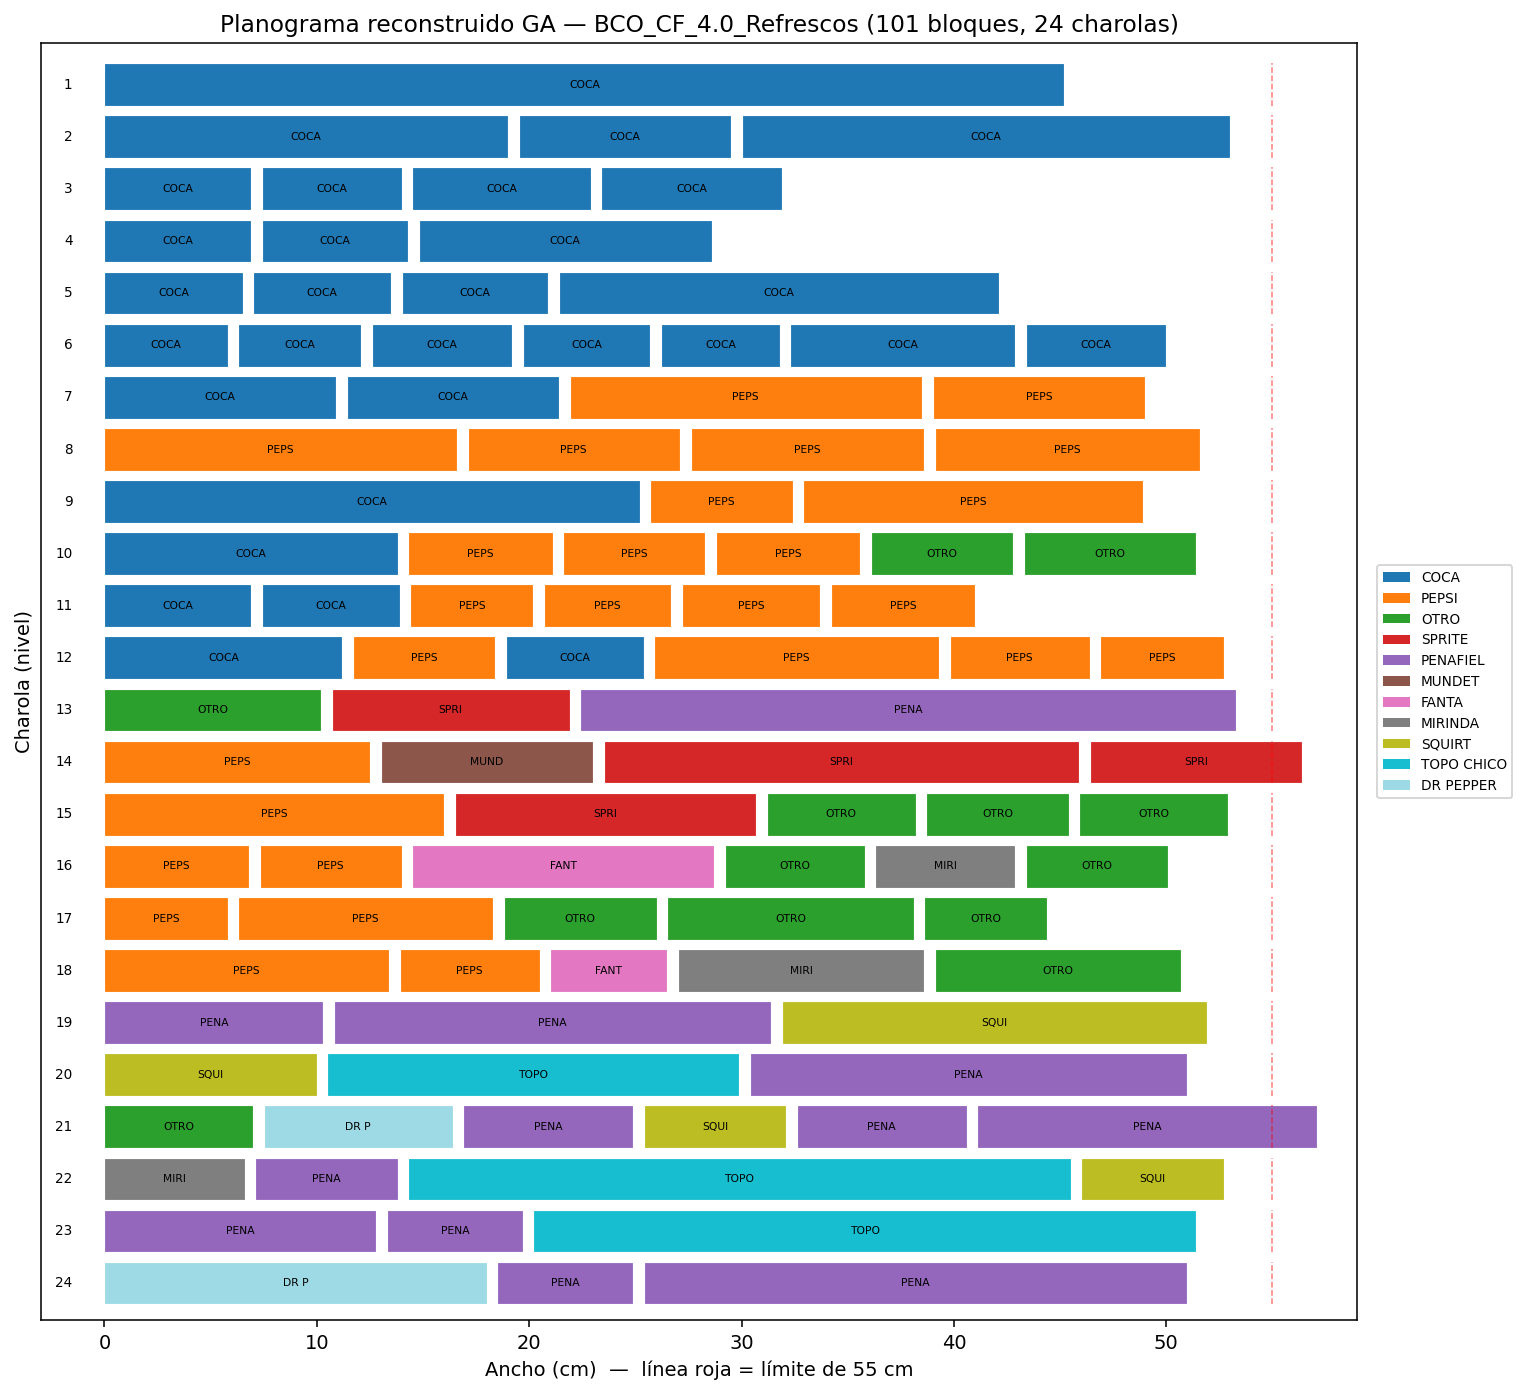
\includegraphics[width=0.9\textwidth]{planograma_bco.png}
\caption{Planograma reconstruido por el GA para \texttt{BCO\_CF\_4.0\_Refrescos}
(101 bloques, 24 charolas). La l\'inea roja marca el l\'imite de 55 cm.}
\label{fig:plano}
\end{figure}

\subsection{Convergencia y comparaci\'on por criterio}
\begin{figure}[H]
\centering
\begin{subfigure}{0.48\textwidth}
  \centering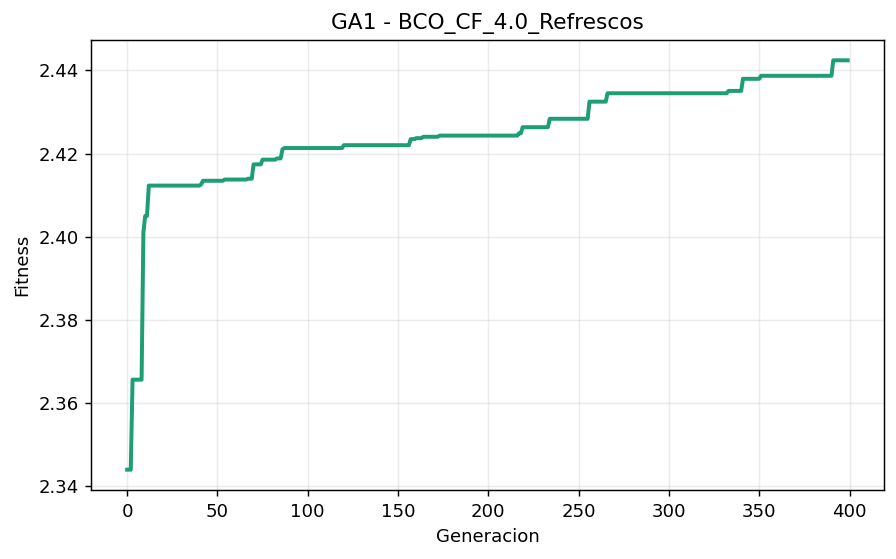
\includegraphics[width=\textwidth]{resultados_ga1.png}
  \caption{GA1 (no extendido).}
\end{subfigure}\hfill
\begin{subfigure}{0.48\textwidth}
  \centering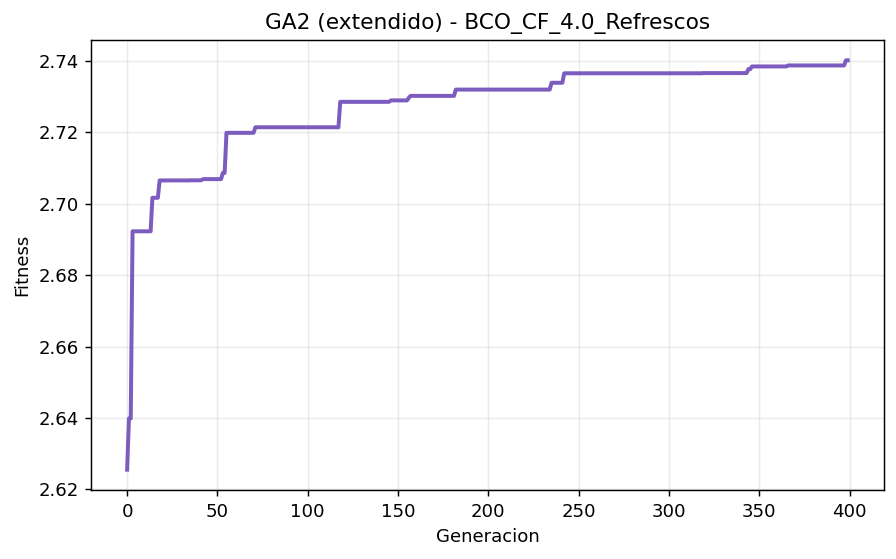
\includegraphics[width=\textwidth]{resultados_ga2.png}
  \caption{GA2 (extendido, con t\'ermino $w_4$).}
\end{subfigure}
\caption{Convergencia del fitness de las dos variantes del algoritmo gen\'etico en
\texttt{BCO\_CF\_4.0\_Refrescos}.}
\label{fig:conv-ga}
\end{figure}

\begin{figure}[H]
\centering
\begin{subfigure}{0.48\textwidth}
  \centering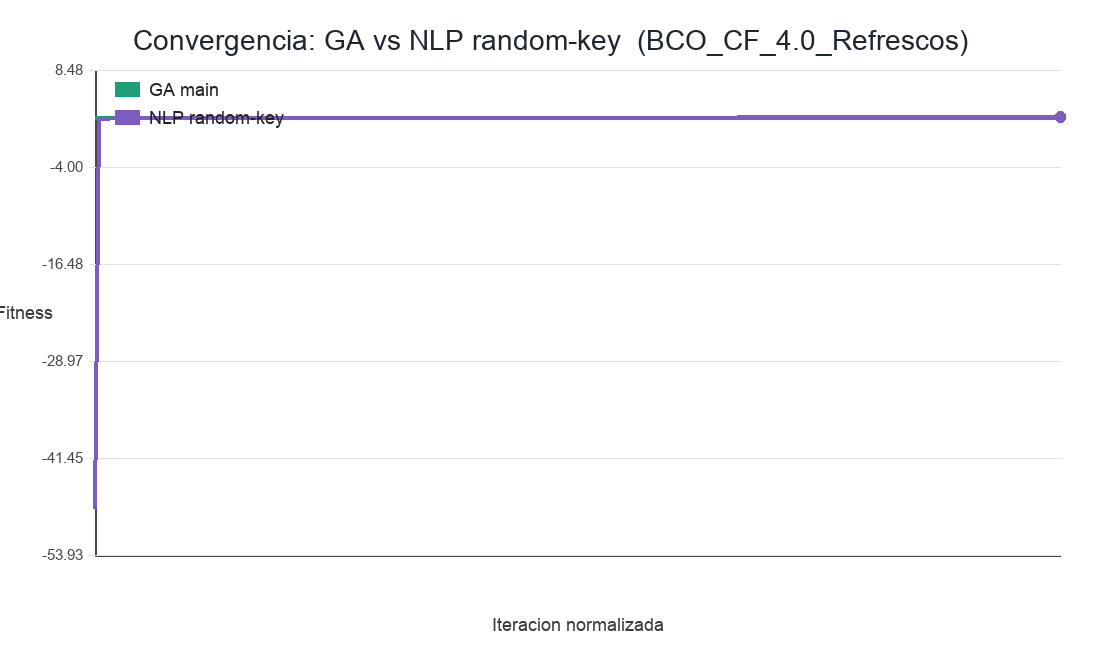
\includegraphics[width=\textwidth]{convergencia_BCO_CF_4.0_Refrescos.png}
  \caption{Convergencia GA vs.\ NLP.}
\end{subfigure}\hfill
\begin{subfigure}{0.48\textwidth}
  \centering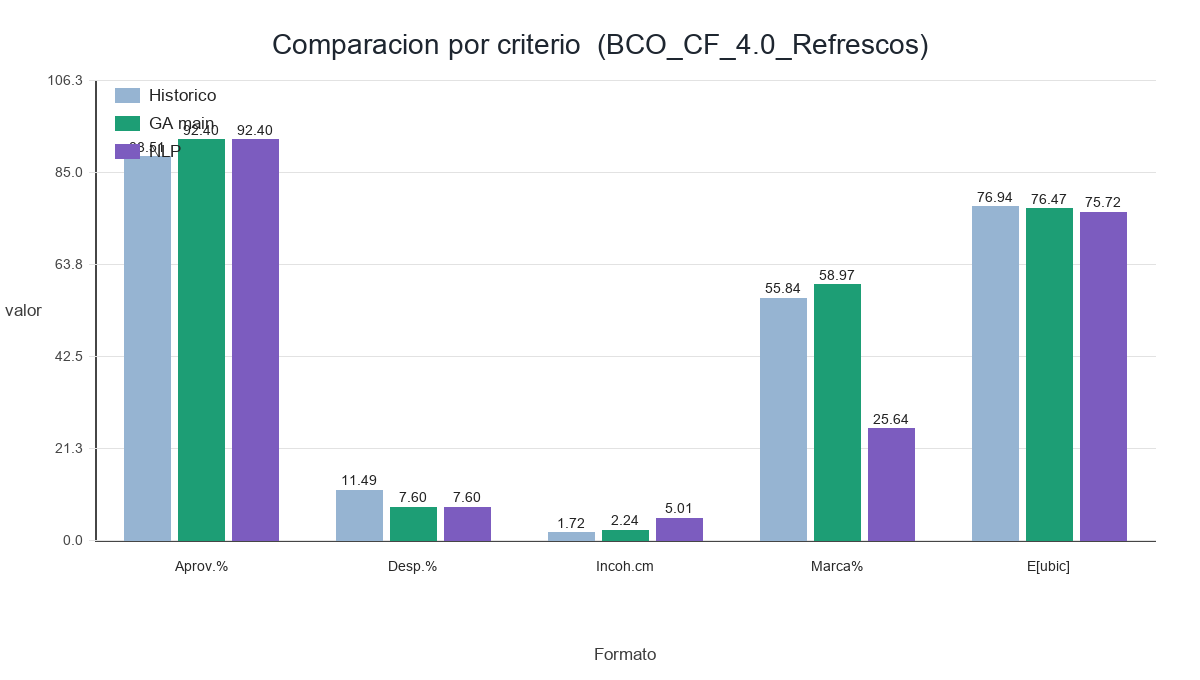
\includegraphics[width=\textwidth]{criterios_BCO_CF_4.0_Refrescos.png}
  \caption{Comparaci\'on por criterio.}
\end{subfigure}
\caption{Izquierda: el GA converge a un mejor fitness que la evoluci\'on diferencial
sobre las llaves continuas. Derecha: ambos igualan el aprovechamiento, pero el GA
mantiene mucho mejor la agrupaci\'on de marca y la coherencia de tama\~no.}
\label{fig:comp-fig}
\end{figure}

% ======================================================================
\section{Conclusiones}
% ======================================================================
\begin{itemize}[leftmargin=1.6em, itemsep=0.3em]
\item El modelo de planogramaci\'on produce acomodos v\'alidos en los cuatro formatos,
con aprovechamiento de 90.9\,\% a 95.7\,\%, respetando las restricciones f\'isicas y
el espaciado de 0.5 cm.
\item \textbf{El algoritmo gen\'etico supera al acomodo experto hist\'orico y al
modelo no lineal en los cuatro formatos.} El NLP iguala el aprovechamiento pero pierde
en coherencia de tama\~no y agrupaci\'on de marca, y adem\'as consume m\'as tiempo y
evaluaciones. Esto valida emp\'iricamente la elecci\'on del GA.
\item La reconstrucci\'on por bloques-producto permiti\'o trabajar con planogramas
realistas (27 a 156 bloques) en lugar del universo agregado del formato.
\item Los valores esperados de ubicaci\'on y los pesos de la funci\'on objetivo se
derivaron de los datos por simulaci\'on, no se fijaron a mano.
\item El modelo es parametrizable: cambiar $W$ de 55 a 91 cm lo extiende a g\'ondola
central sin reformular.
\item \textbf{Limitaci\'on:} el planograma modal es una aproximaci\'on estad\'istica;
unas pocas charolas exceden ligeramente 55 cm (m\'ax 57.1 en \texttt{BCO\_CF\_4.0},
2 de 24), artefacto de mezclar modas de distintas tiendas.
\item \textbf{Factibilidad de la extensi\'on:} GA2 est\'a preparado para incorporar
par\'ametros reales (demanda, margen) cuando el socio los proporcione; actualmente se
usan valores \emph{placeholder}.
\end{itemize}

% ======================================================================
\section*{Anexo: c\'odigo}
\addcontentsline{toc}{section}{Anexo: c\'odigo}
% ======================================================================
C\'odigo disponible en el repositorio
\href{https://github.com/DanielLaBanda/RETO_OXXO_OPTINL}{\texttt{DanielLaBanda/RETO\_OXXO\_OPTINL}}.
Archivos principales:
\begin{itemize}[leftmargin=1.6em, itemsep=0.15em]
\item \texttt{preprocessing/pipeline\_.py} --- reconstrucci\'on de planogramas y
simulaci\'on de pesos.
\item \texttt{genetic\_algorithm/ga1.py} y \texttt{ga2.py} --- modelos no extendido y
extendido.
\item \texttt{mathematical\_model/nlp\_model.py} --- modelo no lineal random-key y
comparaci\'on contra el GA.
\item \texttt{mathematical\_model/math\_model.py} --- generaci\'on de tablas y
figuras de resultados.
\end{itemize}

% ======================================================================
\section*{Bibliograf\'ia}
\addcontentsline{toc}{section}{Bibliograf\'ia}
% ======================================================================
\begin{thebibliography}{9}
\bibitem{hubner2016} H\"ubner, A.\ y Schaal, K.\ (2016). A shelf-space optimization
model when demand is stochastic and space-elastic. \emph{Omega}, 68, 139--154.
\bibitem{czerniachowska2021} Czerniachowska, K.\ et al.\ (2021). Genetic algorithm
for the retailers' shelf space allocation profit maximization problem.
\emph{Applied Sciences}, 11(14), 6401.
\bibitem{gencosman2021} Gencosman, B.\,C.\ y Begen, M.\,A.\ (2021). Exact optimization
and decomposition approaches for shelf space allocation. \emph{European Journal of
Operational Research}, 299(2), 432--447.
\bibitem{storn1997} Storn, R.\ y Price, K.\ (1997). Differential Evolution --- a
simple and efficient heuristic for global optimization over continuous spaces.
\emph{Journal of Global Optimization}, 11(4), 341--359.
\bibitem{isa2024} Isa, F.\,M.\ et al.\ (2024). Shelf space allocation problem (SSAP)
in the retail industry: A systematic literature review.
\end{thebibliography}

\end{document}
